\documentclass[a4paper,11pt,twocolumn]{article}

\usepackage{xltxtra}
\usepackage{fontspec}

\defaultfontfeatures{Scale=MatchLowercase,Mapping=tex-text}

\usepackage{times}
\usepackage{natbib}

\usepackage[small,bf]{caption}


\setmainfont[BoldFont={Times New Roman}]{Times New Roman}
\setromanfont{Times New Roman}
%\setmonofont{FreeMono}


\bibdata{paper}


\title{A North Sámi to South Sámi machine translation prototype}
\author{Lene Antonsen,\\Giellatekno,\\Tromsø\\{\tt lene.antonsen@uit.no}
\and Francis Tyers,\\Giellatekno,\\Tromsø\\{\tt ftyers@dlsi.ua.es}
\and Trond Trosterud,\\Giellatekno,\\Tromsø\\{\tt trond.trosterud@uit.no}}
\date{}

\begin{document}

\maketitle

\section{Introduction}
%@trond
%To be written after the paper is finished, but try to state the idea.

The paper presents a machine translation system from North Saami to
South Saami. The system is intended to work in a translation setting
where North Saami acts as a pivot language, with manual translation
from Norwegian into the largest of the Saami languages, and thereafter
to offer machine translation service, with postediting, to the other,
smaller, Saami languages. On the one hand, the Saami languages are
closely related, and therefore lend themselves better to MT than a
system translating from Norwegian directly, but on the other hand, the
classical problems of translating via a pivot language apply in this
case as well. 

The paper is structured as follows. Afther looking at previous work
and at the languages themselves, we give a presentation of the actual
machine translation system. Thereafter comes an evaluation of the
system. We presented translated text to translators, alongside with
the Norwegian original, without revealing the fact that the texts were
actually translated from North Saami.

finally comes a conclusion.


% Previous work
\cite{tyers09} \cite{wiechetek10} \cite{trosterud12}
% LREC?

%pivot translation references --babych paper
\cite{babych2007}

\section{Languages}
%@trond
% [Sámi language area map]

Norwegian North Germanic. The Saami languages constitute the
westernmost branch of the Uralic language family. They possess most of
the classical Uralic characteristica: A rich verbal morphology (3
numbers and persons, a rich repertoire of infinite forms), and a
medium-size case system with both grammatical and adverbial functions,
and no gender distinction. They also show extensive contact with their
Germanic neighbours. Many grammatical structures are head-initial
constructions, as compared to the classical Uralic pattern, and the
tense system is compatible with the North Germanic one.

North and South Saami are not mutually intellegible, due both to
linguistic distance and to radically different prinicples for their
literary languages. An analogy would be the difference between English 
and Frisian. 

Grammatical similarities between North and South Saami include the 
following: Both languages have 3 persons and numbers, they have a similar
system for postpositions and verb derivation. Noun phrase syntax is 
similar, and the case systems are almost identical.

Taking a closer look, there are still differences. In both North and
South Saami, negation is expressed with a negation verb which inflects
for person and number, but in 
South Saami, this verb is inflected for Tense as well. South Saami
has OV word order and lacks a copula in predicative constructions, 
whereas North Saami uses VO in simple sentences, and requires a copula.

Although the case systems are similar, North Saami has a locative case
that covers the semantic field of both inessive and elative in 
South Saami, the locative must thus be split into two cases. There is
also some differences in case usage, plural objects are accusative
in North Saami, but nominative for indefinite and accusative for 
definite objects in South Saami.

For a machine translation system the orthographic differences 
imply that apart from person
names and acronyms there will be no free rides during the conversion 
process. The core vocabulary is distinct, even recent loans from
the same donor languages are different, and the vocabulary coverage
for a working system must thus be very good.

An overview over the differences between the two languages can
be found in \cite{sammallahti98}.


\section{Implementation}
%@fran
% [Pipeline image]

The translator was implemented using the Apertium platform \cite{forcada2011}. Apertium 
provides a highly modular set of tools for building rule-based
machine translation systems. Apertium language pairs are set up as Unix pipelines, where the
typical pipeline consists of:

\begin{itemize}
\item deformatting (encapsulating formatting/markup from the engine),
\item source-language (SL) morphological analysis with a finite-state
  transducer (FST),
\item disambiguation using a Hidden Markov Model (HMM) and/or
  Constraint Grammar (CG), 
\item lexical transfer (word-translation on the disambiguated source),
\item lexical selection (choosing the appropriate word out of a set of possible
   translations),
\item one or more levels of finite-state based structural transfer
  (reordering, and changes to morphological features),
\item target-language (TL) generation with an FST
\item reformatting (unencapsulating format information)
\end{itemize}

See Figure~\ref{fig:pipeline} for an overview of the modules used
in this particular language pair.

\begin{figure*}
 \centering
 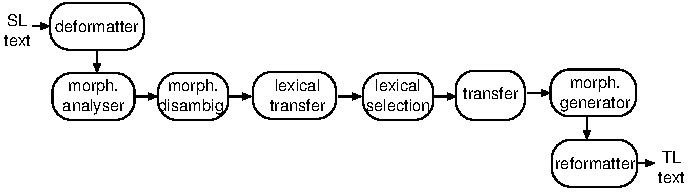
\includegraphics[width=0.75\textwidth]{architecture-overview.pdf}
 \caption{Overview of the translation pipeline.}
 \label{fig:pipeline}
\end{figure*}

\subsection{Analysis}

Morphological analysis is done on the input using the Helsinki Finite-State
Toolkit \cite{linden2011}. For each surface form, a finite-state transducer
returns a set of the possible analyses, where an analysis is a combination
of lemma, and a sequence of tags which describe the morphological structure
of the surface form.

A Constraint Grammar-based disambiguator then selects the most appropriate 
analysis for each surface form according to the context, and assigns to each 
analysis a syntactic tag denoting its syntactic function (subject, object, 
main verb, \ldots).

\subsection{Transfer}

\subsubsection{Lexical transfer}

Large syntactic differences also have consequences for the bidix, because there are many examples of sme-verb has go be translated into object+verb og adverb+verb in sma.
ex: nob `å trekke lodd' sme \textit{vuorbádit} sma \textit{vuerpiem giesedh}, 
nob `å presentere' sme \textit{ovdanbuktit} sma \textit{åvtese buektedh}. 
I mange tilfeller er grunnen til denne  forskjellen at man på sme har fått utviklet flere termer som matcher de norske teremene, mens man på sma
fremdeles må forklare innholdet.



The bilingual dictionary
general dictionary
general words
special domain

\textbf{Problems caused by this model: ex from two terms to one term to two terms}

Example: nob-1,2   sme-x   sma-1,2
example the verbs ‘read, count, say’, nob: \textit{lese, telle, uttale}, sme: \textit{lohkat} can be used about all three, sma: \textit{lohkedh, ryöknehtidh, jiehtedh} 

Little nob-sma lexical resources, and total lack of sme-sma, we have to find words by comparing translated texts (nob-sme with nob-sma)

\textbf{Problems combining sma-nob and sme-nob dictionary}
This was done, it had to be manually edited because of nob-words with more than one meaning. 
Example: nob \textit{regne} means both 'to rain' and ‘to calculate’, 
which are two different verbs both in sme \textit{arvit, rehkenastit} and in sma \textit{abrodh, ryöknedh}

\subsubsection{Lexical selection}

\subsubsection{Structural transfer}

The syntactic differences between North Saami and South Saami are
greater than are usually dealt with between related language pairs
in Apertium. 
In order to be able to transfer VO structures to OV more reliably,
the transfer phase is split into five parts instead of the three
more typically used in Apertium:

%t1x local chunking NP, VP
%t2x localcoordination NP+NP, etc.
%t3x empty, but for adpositional phrases + Rel clauses
%t4x Constituent mvm, SVO -> SOV
%t5x Cleanup


\begin{itemize} 
  \item \texttt{chunker}: Chunk input words into groups, e.g. noun groups, verb chains
  \item \texttt{interchunk1}: Merge chunks which have local coordination, e.g. the sequence [NP $x$] [CC and] [NP $y$] is merged into [NP $x$ and $y$]
  \item \texttt{interchunk2}: Merges relative clauses and adpositional phrases.
  \item \texttt{interchunk3}: Reorder constituents, e.g. SVO $\rightarrow$ SOV.
  \item \texttt{postchunk}: Cleanup
\end{itemize}


\subsubsection{Generation}

Generation is done using a finite-state transducer, also 
compiled using HFST. Each lexical unit which is output by
the postchunk module is looked up in the generation transducer
and the surface form is output.

\section{Evaluation}
%@ lene,fran
 translation nob-sma which actually is nob-sme-sma (should somehow be in the title?) 
 the evaluators evaluate nob-sma

\subsection{Statistics}
%@fran
\begin{table}
  \begin{center}
    \begin{tabular}{|l|r|}
      \hline
      Bilingual dictionary ({\tt sme}$\rightarrow${\tt sma}) & 15,204 \\ % 10776 proper names
      Transfer rules ({\tt sme}$\rightarrow${\tt sma}) & 57 \\
      \hline
    \end{tabular}
    \label{table:transfer}
    \caption{Number of bilingual dictionary entries and transfer rules}
  \end{center}
\end{table}

\begin{table}
  \begin{center}
    \begin{tabular}{|l|r|r|}
      \hline
      \textbf{Corpus} & \textbf{Tokens} & \textbf{Coverage (\%)}  \\
      \hline
      Schoolbooks     & 468,697 & 92.4 $\pm$ 0.58 \\
      General         & & 0.0 $\pm$ 0.0 \\
      \hline
    \end{tabular}
    \label{table:coverage}
    \caption{Vocabulary coverage of the system}
  \end{center}
\end{table}

\subsection{Quantitative}
%@lene
\subsection{Qualitative}
%@lene

\subsection{User feedback}
%@lene

\section{Future work}
%@trond
\section{Conclusions}
%@trond

 reaction from sma linguist in the normgiving organ: she sees the possibility of using MT as a help for discussing terminology and getting the best ones into use

 the language socity is used to the impact from the mojority languages, a new controversial(?) thought is the linguistic impact from another minority lanugage 


\section*{Acknowledgements}

Linda Wiechetek, Divvun

\bibliographystyle{apalike}
\bibliography{paper}


\end{document}
